\documentclass{beamer}
\usepackage{graphicx}
\usepackage{listings} % Syntax highlighing
\usepackage{fancyvrb} % Inline verbatim
\usepackage{attachfile}
\usepackage{hyperref} % Hyperlinks
\hypersetup{pdfpagemode=FullScreen}
\usepackage{tikz}
\def\checkmark{\tikz\fill[scale=0.4](0,.35) -- (.25,0) -- (1,.7) -- (.25,.15) -- cycle;}

\usetheme{Boadilla}
\title{Malware Networks, Shared Code}
\author{UMBC Malware Data Science}
\date{Week 3: 11 February 2020}

\begin{document}

\begin{frame}{Recap}
    Last week, we discussed some features pertaining to malware, fuzzy hashes, and the pefile module in Python. Next, we'll take a look at what can be done with such features.
\end{frame}

\begin{frame}{Lab 2}
    \only<1>{
        The three files:
        \begin{itemize}
            \item \texttt{pi}: Simple $\pi$ calculator
            \item \texttt{pi\_debug}: Includes the program's source code
            \item \texttt{pi\_upx}: UPX-packed version of the first file. Smaller file size, actual functionality hidden until execution.
        \end{itemize}
    }
    \only<2>{
        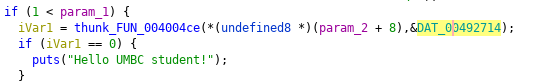
\includegraphics[scale=0.7]{LabAnswers/Lab2Secret1.png}
    }
    \only<3>{
        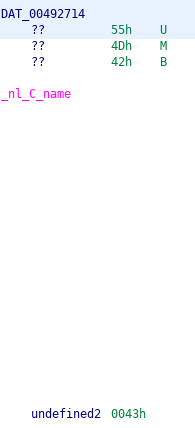
\includegraphics[scale=0.5]{LabAnswers/Lab2Secret1a.png}
    }
    \only<4>{
        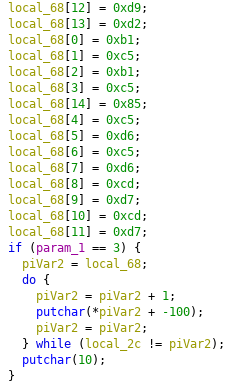
\includegraphics[scale=0.5]{LabAnswers/Lab2Secret2.png}
    }
    \only<5>{
        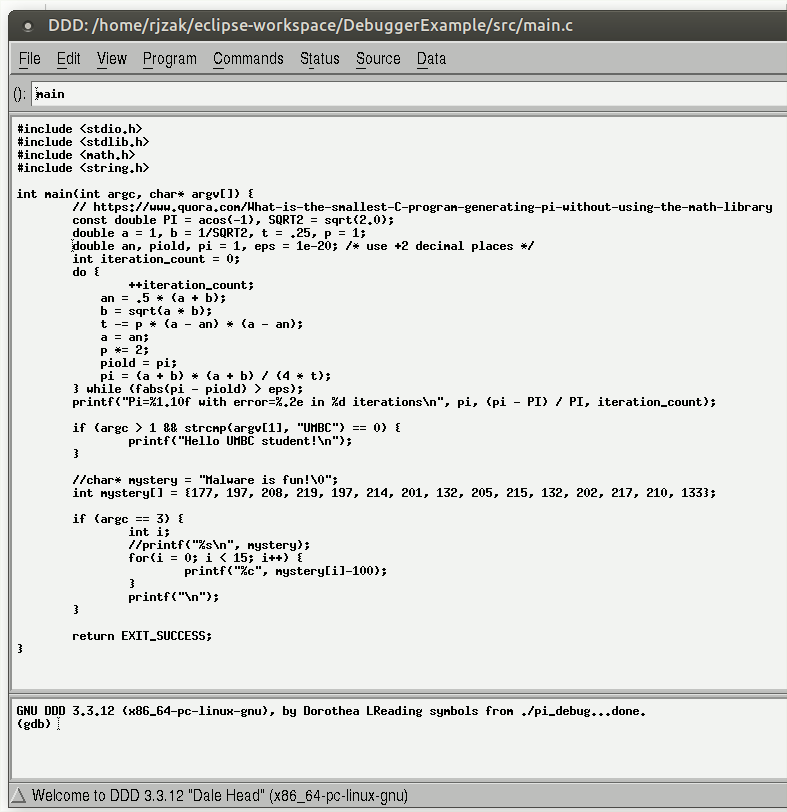
\includegraphics[scale=0.285]{LabAnswers/Lab2ddd.png}
    }
    \only<6>{
        The first argument had to be ``UMBC'', but the second argument could be anything. \\
        \texttt{\$ ./pi UMBC 123} \\
        \texttt{Pi=3.1415926536 with error=2.83e-16 in 4 iterations} \\
        \texttt{Hello UMBC student!} \\
        \texttt{Malware is fun!}
    }
    
\end{frame}

\begin{frame}{Networks}
    Networks are made up of nodes and edges. Nodes represent objects of interest, and edges are the relationship between the objects.
    \\ ~~ \\
    Some of the static features in malware can be used as edges in a network, revealing relationships between seemingly unique malware samples, including hostnames and IP addresses, as shown in Chapter 4. Different malware samples connecting to the same Command \& Control (C2) server likely means the malware is related.
\end{frame}

\begin{frame}{Network Examples}
    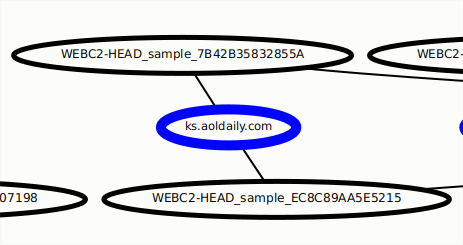
\includegraphics[scale=0.5]{Images/network_good.png}
    \\
    A connection between two separate samples is shown.
\end{frame}

\begin{frame}{Network Examples}
    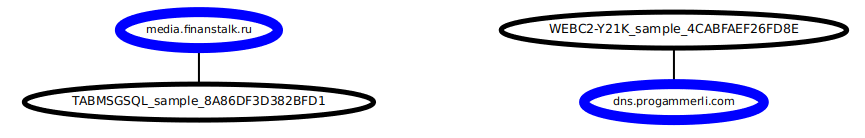
\includegraphics[scale=0.4]{Images/network_not_helpful.png}
    \\
    Two samples, two domains. No clear connection.
\end{frame}

\begin{frame}{Network Examples}
    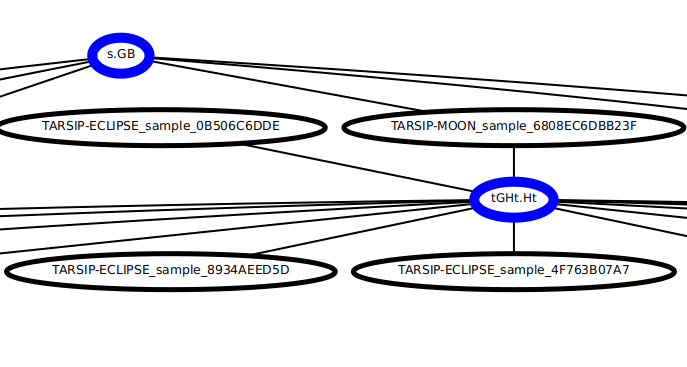
\includegraphics[scale=0.4]{Images/network_useless.png}
    \\
    Connections based on invalid domains. It's important to double-check your code.
\end{frame}

\begin{frame}{Networks}
    Instead of trying to parse out specific data types as points of comparison, such as hostnames, we can look at file characteristics. A fuzzy hash can be used to show similarity. The textbook introduces the Jaccard distance, which is another way to show similarity. A benefit of this is it works on any file type. Without code changes, comparisons instead could be done on PDF malware, for example.
    \\ ~~ \\
    Something like this could be harder for an adversary to change, it would require reworking their code; and one of our goals is to increase the costs for the malware author(s) to evade detection \& analysis.
\end{frame}

\begin{frame}{Network Examples}
    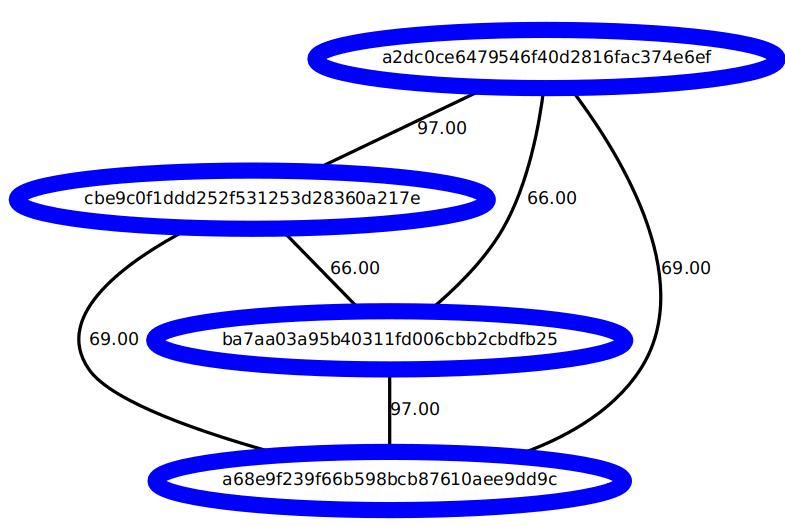
\includegraphics[scale=0.3]{Images/network_ssdeep.png}
    \\
    A network based on SSDeep showing a cluster of related samples. They could be different versions of the same malware, or examples where similar code was used between malware samples.
    %A fuzzy hash might be more reliable at showing similarity, but is costly to compute: $O(n^2)$
\end{frame}

\begin{frame}{Network Examples}
    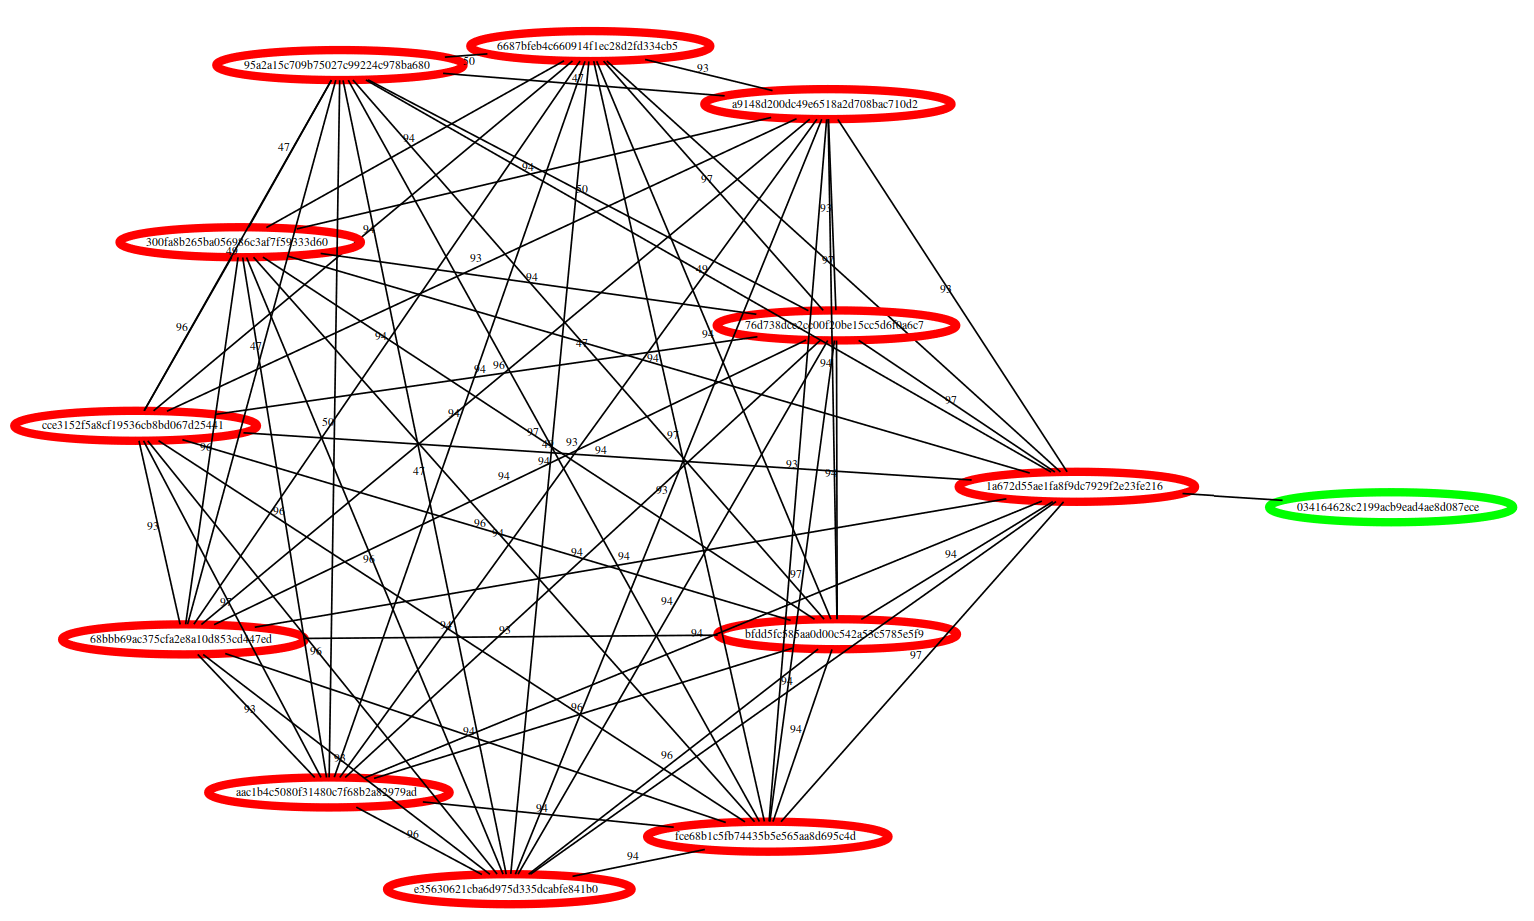
\includegraphics[scale=0.21]{Images/network_goodware.png}
    \\
    A file marked as benign by VirusTotal is related to a cluster of malware, as shown by SSDeep similarity.
\end{frame}

\begin{frame}{Lab 3}
    For this week's Lab, try your hand at creating your own malware relationship network. What are good attributes to link samples to each other? What are some shortcomings to the book's example code?
    \\ ~~ \\
    A note about VMs: you may find that running code on the malware/goodware data in the VM is slow. Where needed, adjust your training and testing sizes so that the code runs in a reasonable amount of time, and document what these data sizes are. Allocating more CPU cores and RAM will improve performance, but this is dependant on your hardware.
    \\ ~~ \\
    For next week, read the papers on use of $n$-grams and machine learning \attachfile{Papers/investigation_byte_ngrams.pdf} \attachfile{Papers/what_can_ngrams_learn.pdf}.
\end{frame}


\end{document}